% Contributions are much appreciated, in order to contribute to this project, head over to this repository:
% https://github.com/bshramin/uofa-eng-assignment

\documentclass[11pt,letterpaper]{article}
\textwidth 6.5in
\textheight 9.in
\oddsidemargin 0in
\headheight 0in
\usepackage{graphicx}
\usepackage{fancybox}
\usepackage[utf8]{inputenc}
\usepackage{epsfig,graphicx}
\usepackage{multicol,pst-plot}
\usepackage{pstricks}
\usepackage{amsmath}
\usepackage{amsfonts}
\usepackage{amssymb}
\usepackage{eucal}
\usepackage[left=2cm,right=2cm,top=2cm,bottom=2cm]{geometry}
\usepackage{esvect}
\pagestyle{empty}
\DeclareMathOperator{\tr}{Tr}
\newcommand*{\op}[1]{\check{\mathbf#1}}
\newcommand{\bra}[1]{\langle #1 |}
\newcommand{\ket}[1]{| #1 \rangle}
\newcommand{\braket}[2]{\langle #1 | #2 \rangle}
\newcommand{\mean}[1]{\langle #1 \rangle}
\newcommand{\opvec}[1]{\check{\vec #1}}
\renewcommand{\sp}[1]{$${\begin{split}#1\end{split}}$$}

\usepackage{lipsum}

\usepackage{listings}
\usepackage{color}
\usepackage{wrapfig}
\usepackage[shortlabels]{enumitem}

\definecolor{codegreen}{rgb}{0,0.6,0}
\definecolor{codegray}{rgb}{0.5,0.5,0.5}
\definecolor{codepurple}{rgb}{0.58,0,0.82}
\definecolor{backcolour}{rgb}{0.95,0.95,0.92}

\lstdefinestyle{mystyle}{
	backgroundcolor=\color{backcolour},   
	commentstyle=\color{codegreen},
	keywordstyle=\color{magenta},
	numberstyle=\tiny\color{codegray},
	stringstyle=\color{codepurple},
	basicstyle=\footnotesize,
	breakatwhitespace=false,         
	breaklines=true,                 
	captionpos=b,                    
	keepspaces=true,                 
	numbers=left,                    
	numbersep=5pt,                  
	showspaces=false,                
	showstringspaces=false,
	showtabs=false,                  
	tabsize=2
}

\lstset{style=mystyle}

\begin{document}
\pagestyle{plain}

\begin{flushleft}
Estudiante: Fabio Quimbay\\
Email: fabio.quimbay883@comunidadunir.net\\
Profesor: Miguel Ángel Cabeza\\
Fecha: Noviembre 7 de 2022\\
\end{flushleft}

\begin{flushright}\vspace{-20mm}

\includegraphics[height=2cm]{logo.png}
\end{flushright}
 
\begin{center}\vspace{0cm}
\textbf{\large PER5786 2022-2023  Física 1 (GFI) - PER5786 2022-2023}\\
 Tema 2 - Cinemática
\end{center}

 
\rule{\linewidth}{0.1mm}
%%%%%%%%%%%%%%%%%%%%%%%%%%%%%%%%%%%%%%%%%%%%%%%%%%%%%%%%%%%%%%%%%%%%%%%%

\bigskip
\bigskip

%%%%%%%%%%%%%%%%%%%%
\textbf{Ejercicio 5 propuesto}\\

\begin{wrapfigure}{r}{0.30\textwidth}
    \centering
    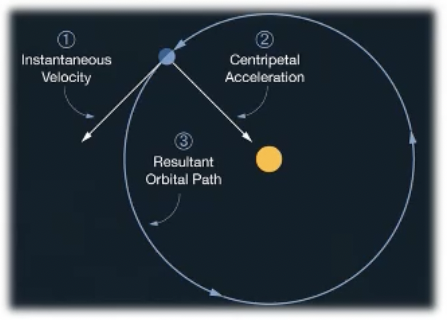
\includegraphics[width=0.25\textwidth]{ejemplo_5.png}
\end{wrapfigure}

Un satélite está orbitando alrededor de la Tierra a una altitud h = 150 km sobre la superficie, donde la aceleración centrípeta es de $9.4\,m/s^2$. El radio de la Tierra es $R = 6,4 \cdot 10^6\,m$. ¿Cuál es la velocidad orbital y el período del satélite?\\

\textbf{Formulas base:}\\

Se tomarán las siguientes formulas base:

\begin{align}
\boxed{ T = \frac{2\pi}{\omega}}\\
\boxed{ V_{LINEAL} = \omega \cdot r}
\end{align}

\textbf{Solución:}\\

Primero es necesario realizar algunas conversiones para establecer las magnitudes en las mismas unidades, a saber:

\begin{align}
r &= 150\,k = 1.5 \times 10^5 m\\
a_{c} &= 9.4\,m/s^2\\
R &= 6.4 \times 10^6\,m
\end{align}

Para obtener la Velocidad Orbital ($V_{ORB}$) despejamos en la ecuación:\\

\begin{align*}
V_{ORB} &= \sqrt{a_{c} \cdot r}\\
V_{ORB} &= \sqrt{9.4\,m/s^2 \cdot (1.5 \times 10^5\,m + 6.4 \times 10^6\,m)}\\
V_{ORB} &= 7846.66\,m/s
\end{align*}

Para poder determinar el periodo (T) es necesario primero determinar la frecuencia angular ($\omega$), así:.\\

\begin{align*}
\omega &= \frac{V_{ORB}}{R_{TOTAL}}\\
\omega &=\frac{7846.66\,m/s}{6.55 \times 10^6\,m} = 0.001198\,rad/s\\
\omega &=1.198 \times 10^{-3}\,rad/s
\,\\ \,\\
T &= \frac{2\cdot\pi}{\omega} = \frac{2\cdot\pi}{1.198 \times 10^{-3}}\\
T &= 5255.73\,s 
\end{align*}

De tal forma, la velocidad orbital ($V_{ORB}$) y el periodo (T) son respectivamente, $7846.66\,m/s$ y $5244.73\,s$.

%%%%%%%%%%%%%%%%%%%%

\end{document}

